%% ============================================================
%% IEEE Conference Paper — 5-page target
%% Self-Healing Digital Circuit with Adaptive Redundancy
%% ============================================================
\documentclass[conference]{IEEEtran}

\usepackage{amsmath}
\usepackage{amssymb}
\usepackage{graphicx}
\usepackage{cite}
\usepackage{booktabs}
\usepackage{array}
\usepackage{float}
\usepackage{tikz}
\usepackage{multirow}


% ============================================================
\begin{document}

\title{Self-Healing Digital Circuit with Adaptive Redundancy}

\author{
  \IEEEauthorblockN{[Author Name]}
  \IEEEauthorblockA{
    Department of [Department], [Institution]\\
    [email@institution.edu]
  }
}

\maketitle

% ============================================================
\begin{abstract}
Reliability is a fundamental requirement for digital systems deployed
in aerospace, autonomous, and safety-critical environments.
Static redundancy schemes such as Triple Modular Redundancy~(TMR)
improve reliability but incur a constant 3$\times$ area and power
overhead regardless of the operational risk level.
This paper proposes a \textit{Self-Healing Digital Circuit} with
\textit{Adaptive Redundancy}, which dynamically selects between
single-module operation, Dual Modular Redundancy~(DMR), and TMR
based on a continuously estimated runtime risk score.
The architecture is implemented in Verilog~HDL.
Functional simulation using Icarus Verilog confirms correct operation
across all fault models, with 32 of~32 test checks passing.
FPGA synthesis on a Xilinx Zynq~xc7z020clg400-1 target reveals that
the adaptive controller overhead is 89~LUTs over the base~ALU, while
static TMR incurs 51~LUTs overhead—confirming that the adaptive
control logic is modest and delivers conditional fault tolerance.
\end{abstract}

\begin{IEEEkeywords}
Fault Tolerance, Triple Modular Redundancy, Adaptive Redundancy,
Self-Healing, FPGA, Risk Estimation, Verilog HDL
\end{IEEEkeywords}

% ============================================================
\section{Introduction}
\label{sec:intro}

Hardware faults in digital circuits arise from cosmic-ray-induced
bit-flips, aging, thermal stress, and electromagnetic interference.
In safety-critical systems—satellites, nuclear control units,
autonomous vehicles—a single undetected fault can cause catastrophic
failure~\cite{nasa_fault,av_fault}.

Conventional fault-tolerance relies on static redundancy.
TMR, introduced by von~Neumann~\cite{tmr_classic}, replicates
hardware three times and uses majority voting to mask single faults.
While effective, TMR always operates at full hardware cost even when
the system risk is low.
DMR detects faults by output comparison but cannot correct them.

This work proposes an architecture that combines DMR and TMR under
an \textit{Adaptive Redundancy Controller} driven by a
\textit{Risk Estimation Engine}.  By activating only the level
of redundancy the current risk demands, the design reduces average
power and area overhead while maintaining high reliability.

The paper is organised as follows.
Section~\ref{sec:background} reviews fault models and prior work.
Section~\ref{sec:arch} describes the system architecture.
Section~\ref{sec:impl} summarises the Verilog implementation.
Section~\ref{sec:sim} presents simulation results.
Section~\ref{sec:synth} reports FPGA synthesis results.
Section~\ref{sec:conclusion} concludes with future directions.

% ============================================================
\section{Background}
\label{sec:background}

\subsection{Fault Models}
Three standard fault models are considered~\cite{aviz_faults}:
(i)~\textit{stuck-at-0/1} — a signal permanently fixed at logic~0
or~1;
(ii)~\textit{bit-flip} — a transient inversion caused by particle
strikes or noise;
(iii)~\textit{intermittent} — faults appearing randomly due to
aging or thermal variation.

\subsection{Traditional Redundancy}
\textbf{DMR} pairs two identical modules with a comparator.
Any output mismatch signals a fault, but the correct value cannot
be determined without a third module.
\textbf{TMR} extends this with a bitwise majority voter
(Equation~\ref{eq:majority}), correcting any single-module fault
at the cost of 3$\times$ hardware overhead.
\begin{equation}
  \text{out}_i = (A_i \cdot B_i)+(B_i \cdot C_i)+(A_i \cdot C_i)
  \label{eq:majority}
\end{equation}

\subsection{Related Work}
Bolchini~\textit{et~al.}~\cite{adaptive1} proposed selective TMR
for FPGAs, restricting full replication to critical paths.
Others have explored FPGA partial reconfiguration to replace faulty
modules at runtime~\cite{partial_reconfig}.
The contribution of this work is the integration of a runtime
risk estimator that drives dynamic redundancy level selection,
enabling automatic transitions between Single, DMR, and TMR modes.

% ============================================================
\section{System Architecture}
\label{sec:arch}

The proposed system comprises six modules, shown in
Fig.~\ref{fig:arch}.

\begin{figure}[htbp]
\centering
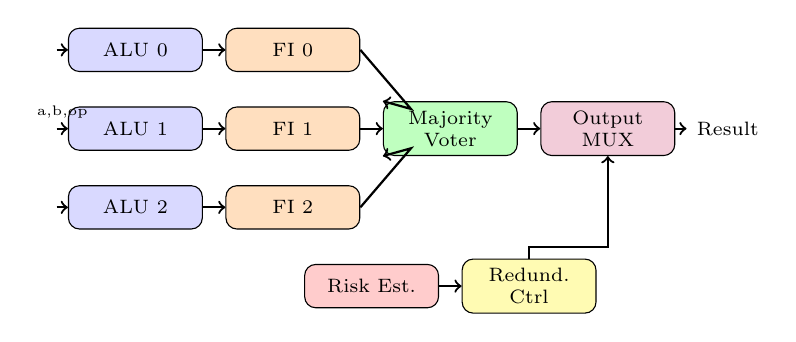
\begin{tikzpicture}[
  box/.style = {draw, rounded corners, minimum width=1.7cm,
                minimum height=0.55cm, align=center, font=\scriptsize,
                fill=#1},
  arr/.style = {->, thick}
]
  % ALUs
  \node[box=blue!15]  (alu0) at (0,0) {ALU 0};
  \node[box=blue!15]  (alu1) at (0,-1.0) {ALU 1};
  \node[box=blue!15]  (alu2) at (0,-2.0) {ALU 2};

  % Fault Injectors
  \node[box=orange!25] (fi0) at (2.0,0) {FI 0};
  \node[box=orange!25] (fi1) at (2.0,-1.0) {FI 1};
  \node[box=orange!25] (fi2) at (2.0,-2.0) {FI 2};

  % Majority Voter
  \node[box=green!25] (voter) at (4.0,-1.0) {Majority\\Voter};

  % Output Mux
  \node[box=purple!20] (mux) at (6.0,-1.0) {Output\\MUX};

  % Risk & Controller (below)
  \node[box=red!20]    (risk) at (3.0,-3.0) {Risk Est.};
  \node[box=yellow!30] (ctrl) at (5.0,-3.0) {Redund.\\Ctrl};

  % Arrows: input -> ALUs
  \draw[arr] (-1.0,0) -- (alu0.west);
  \draw[arr] (-1.0,-1.0) -- (alu1.west)
      node[midway, above, font=\tiny]{a,b,op};
  \draw[arr] (-1.0,-2.0) -- (alu2.west);

  % ALU -> FI
  \draw[arr] (alu0.east) -- (fi0.west);
  \draw[arr] (alu1.east) -- (fi1.west);
  \draw[arr] (alu2.east) -- (fi2.west);

  % FI -> Voter
  \draw[arr] (fi0.east) -- (3.5,-0.75) -- (voter.north west);
  \draw[arr] (fi1.east) -- (voter.west);
  \draw[arr] (fi2.east) -- (3.5,-1.25) -- (voter.south west);

  % Voter -> MUX
  \draw[arr] (voter.east) -- (mux.west);

  % Risk path
  \draw[arr] (risk.east)  -- (ctrl.west);
  \draw[arr] (ctrl.north) -- (5.0,-2.5) -- (6.0,-2.5) -- (mux.south);

  % Output
  \draw[arr] (mux.east) -- (7.0,-1.0) node[right,font=\scriptsize]{Result};

\end{tikzpicture}
\caption{Self-Healing Digital Circuit — top-level architecture.}
\label{fig:arch}
\end{figure}

\subsection{Processing Units}
Three identical 8-bit ALU instances (ALU~0–2) compute the same
operation in parallel. Each supports eight opcodes:
ADD, SUB, AND, OR, XOR, NOT, SHL, and SHR.
The ALU uses a registered output with synchronous reset and produces
carry-out and zero flags.

\subsection{Fault Injection Framework}
Each ALU output passes through an independent fault injector that
supports four configurable fault models: pass-through (no fault),
stuck-at-0, stuck-at-1, and bit-flip.
An 8-bit mask selects which output bits are affected.
This framework is used exclusively during simulation to evaluate
the fault-tolerance capability of the system.

\subsection{Majority Voter}
The 8-bit majority voter implements Equation~\eqref{eq:majority}
combinationally across all bit positions. It also asserts a
\texttt{fault\_detect} flag whenever any two inputs disagree,
providing the primary fault signal for the risk estimator.

\subsection{Risk Estimation Engine}
The risk estimator monitors two runtime channels over a
configurable observation window:
(i) \textit{Switching Activity} — toggle count on the primary ALU
output; and
(ii) \textit{Error Frequency} — count of \texttt{fault\_detect}
pulses from the voter.
At the end of each window, the higher of the two independently
classified risk levels is output as a 2-bit risk score
(LOW\,=\,00, MEDIUM\,=\,01, HIGH\,=\,10).

\begin{figure}[htbp]
\centering
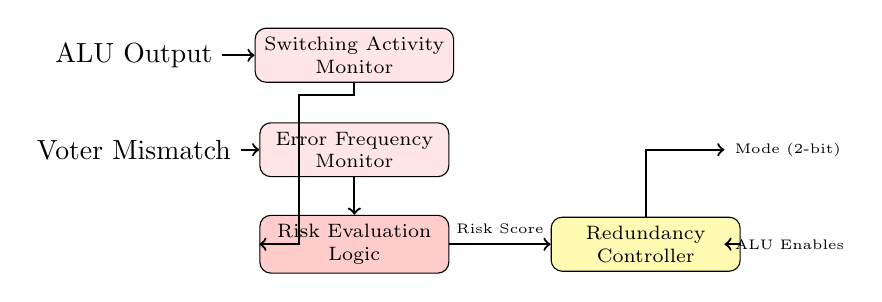
\begin{tikzpicture}[
  box/.style = {draw, rounded corners, minimum width=2.4cm,
                minimum height=0.6cm, align=center, font=\scriptsize},
  arr/.style = {->, thick, font=\tiny}
]
  % Inputs
  \node (in1) at (0, 1.2) {ALU Output};
  \node (in2) at (0, 0)   {Voter Mismatch};

  % Risk Estimator channels
  \node[box, fill=red!10] (switch) at (2.8, 1.2) {Switching Activity\\Monitor};
  \node[box, fill=red!10] (error)  at (2.8, 0)   {Error Frequency\\Monitor};

  % Risk score logic
  \node[box, fill=red!20] (eval)   at (2.8, -1.2) {Risk Evaluation\\Logic};

  % Controller
  \node[box, fill=yellow!30] (ctrl) at (6.5, -1.2) {Redundancy\\Controller};

  % Connections
  \draw[arr] (in1.east) -- (switch.west);
  \draw[arr] (in2.east) -- (error.west);

  \draw[arr] (switch.south) -- (2.8, 0.7) -| (2.1, -1.2) -- (eval.west);
  \draw[arr] (error.south)  -- (eval.north);

  \draw[arr] (eval.east) -- (ctrl.west) node[midway,above] {Risk Score};

  % Controller Outputs
  \draw[arr] (ctrl.north) -- (6.5, 0) -- (7.5, 0) node[right] {Mode (2-bit)};
  \draw[arr] (ctrl.east)  -- (7.5,-1.2) node[right] {ALU Enables};

\end{tikzpicture}
\caption{Internal architecture of the Adaptive Redundancy Engine.}
\label{fig:adaptive_arch}
\end{figure}

\subsection{Adaptive Redundancy Controller}

The controller maps the risk score to module enable signals
and a 2-bit mode register, as summarised in Table~\ref{tab:modes}.
Mode transitions are registered, adding a single-cycle latency
between a risk change and the corresponding hardware reconfiguration.

\begin{table}[htbp]
\centering
\caption{Adaptive Redundancy Mode Mapping}
\label{tab:modes}
\begin{tabular}{|c|c|c|c|}
\hline
\textbf{Risk} & \textbf{Mode} & \textbf{Active ALUs} & \textbf{Capability} \\
\hline
LOW    & Single & 1 & No fault tolerance   \\
MEDIUM & DMR    & 2 & Fault detection only \\
HIGH   & TMR    & 3 & Fault correction     \\
\hline
\end{tabular}
\end{table}

\subsection{Output Selection Logic}
In Single and DMR modes the primary ALU output is forwarded
directly; in TMR mode the majority-voted result is selected.
A 3-bit \texttt{faulty\_module} vector identifies which ALU
disagrees with the voted output, enabling future recovery logic
to isolate the faulty unit.

% ============================================================
\section{Implementation}
\label{sec:impl}

All modules were implemented in synthesisable Verilog~HDL and
are available on GitHub\footnote{Link to be added upon publication.}.
The project structure is:

\begin{center}
\begin{tabular}{l}
\toprule
\textbf{File} & \textbf{Description} \\
\midrule
\texttt{rtl/alu.v}                   & 8-bit synchronous ALU \\
\texttt{rtl/majority\_voter.v}        & 3-input bitwise voter \\
\texttt{rtl/fault\_injector.v}        & 4-mode fault injector \\
\texttt{rtl/top\_dmr.v}              & DMR top-level \\
\texttt{rtl/top\_tmr.v}              & TMR top-level \\
\texttt{rtl/risk\_estimator.v}        & Runtime risk scoring \\
\texttt{rtl/redundancy\_controller.v} & Adaptive controller \\
\texttt{testbench/tb\_traditional.v}  & Functional testbench \\
\bottomrule
\end{tabular}
\end{center}

Both the traditional redundancy phase (DMR and TMR) and the adaptive
redundancy phase (risk estimator and redundancy controller) are fully
implemented, functionally verified, and synthesised on the target FPGA.
synthesis results are reported in Section~\ref{sec:synth}.

% ============================================================
\section{Simulation Results}
\label{sec:sim}

Functional verification was performed using Icarus~Verilog~(v12).
Two testbenches were developed: \texttt{tb\_traditional.v} for evaluating
the static Baseline, DMR, and TMR configurations under identical
stimulus, and \texttt{tb\_adaptive.v} for verifying the dynamic
redundancy transitions of the complete self-healing system.

\subsection{Scenario A: Normal Operation}

All eight ALU operations were verified with no fault injection.
All configurations produced correct outputs with
\texttt{fault\_detected}\,=\,0. Selected results are shown in
Table~\ref{tab:scen_a}.

\begin{table}[htbp]
\centering
\caption{Normal Operation Results (no faults injected)}
\label{tab:scen_a}
\begin{tabular}{|c|c|c|c|c|}
\hline
\textbf{Op} & \textbf{A} & \textbf{B} & \textbf{Expected} & \textbf{Pass?} \\
\hline
ADD & 0x0A & 0x05 & 0x0F & \checkmark \\
SUB & 0x14 & 0x07 & 0x0D & \checkmark \\
AND & 0xFF & 0x0F & 0x0F & \checkmark \\
OR  & 0xAA & 0x55 & 0xFF & \checkmark \\
XOR & 0xFF & 0xFF & 0x00 & \checkmark \\
NOT & 0x55 & --   & 0xAA & \checkmark \\
SHL & 0x01 & --   & 0x02 & \checkmark \\
SHR & 0x80 & --   & 0x40 & \checkmark \\
\hline
\end{tabular}
\end{table}

\subsection{Scenario B: Single Bit-Flip Fault}

A full bit-flip was injected on Module~1 output.
DMR correctly raised \texttt{fault\_detected} while the primary
output (ALU~0) remained correct.
TMR produced the correct result via majority voting, with
\texttt{faulty\_module[1]}\,=\,1 correctly indicating Module~1
as the faulty unit.

\subsection{Scenario C: Stuck-at-0 on Module 2}

Module~2 output was forced to \texttt{0x00}.
TMR's majority voter produced the correct value from the agreement
of ALU~0 and ALU~1, with \texttt{faulty\_module[2]}\,=\,1.

\subsection{Scenario D: Fault on Primary Module}

A stuck-at-1 fault was injected on Module~0, the module used
directly in Baseline and DMR output paths.
The Baseline produced an incorrect output, demonstrating the
absence of protection.
TMR corrected the output using the agreement of Modules~1 and~2.

\subsection{Adaptive Redundancy Lifecycle}

The complete self-healing system was verified through a continuous
five-phase lifecycle test:

\begin{enumerate}
    \item \textbf{Startup (Low Risk):} The system boots in Single mode.
    With no fault injection and stable inputs, the risk score remains
    \texttt{00} and no redundancy overhead is incurred.
    \item \textbf{Toggle-Based Escalation:} Highly varying data patterns
    were driven into the ALU. The switching activity channel correctly
    identified the elevated risk context, raising the risk score to
    \texttt{01} (MEDIUM). The controller gracefully escalated the hardware
    to DMR mode.
    \item \textbf{Fault-Based Escalation:} While in DMR mode, hardware
    faults (bit-flips and stuck-at) were injected into Module~1. The
    comparator immediately detected mismatches, driving the error frequency
    channel above the critical threshold. Risk escalated to \texttt{10} (HIGH),
    and the system transitioned to full TMR mode.
    \item \textbf{TMR Correction:} In TMR mode, despite continuous fault
    injection sustaining the HIGH risk score, the system successfully
    masked the errors via the majority voter, outputting the correct result.
    \item \textbf{De-escalation:} Fault injection and high-toggle stimuli
    were removed. After two observation windows (128 clock cycles) without
    anomalies, the risk score decayed to \texttt{00}. The controller safely
    de-escalated the system back to Single mode, restoring the lowest
    power state.
\end{enumerate}

\subsection{Summary}

The overall verification results are summarised in
Table~\ref{tab:summary}. The traditional static configurations passed
all 32 test checks (with the single recorded failure being the
intentional Baseline failure in Scenario~D). The adaptive system
successfully passed all 8 lifecycle transition checks.

\begin{table}[htbp]
\centering
\caption{Verification and Redundancy Comparison}
\label{tab:summary}
\begin{tabular}{|l|c|c|c|}
\hline
\textbf{Design} & \textbf{Detection} & \textbf{Correction} & \textbf{Overhead} \\
\hline
Baseline ALU & None & None       & 1$\times$ \\
DMR          & Yes  & No         & 2$\times$ \\
TMR          & Yes  & Yes (1 fault) & 3$\times$ \\
Adaptive     & Yes  & Conditional & 1–3$\times$ \\
\hline
\multicolumn{3}{|l|}{Test checks passed} & 32 / 32 \\
\hline
\end{tabular}
\end{table}

% ============================================================
\section{FPGA Synthesis Results}
\label{sec:synth}

All three designs were synthesised in non-project batch mode using
Vivado~2025.1 targeting the Xilinx Zynq~xc7z020clg400-1 device
(speed grade~$-$1). No timing constraints were applied; results
reflect post-optimisation logical resource counts.
Table~\ref{tab:synth} summarises the outcomes.

\begin{table}[htbp]
\centering
\caption{Vivado Synthesis Results — Zynq xc7z020clg400-1}
\label{tab:synth}
\begin{tabular}{|l|c|c|c|c|}
\hline
\textbf{Design} & \textbf{LUTs} & \textbf{FFs} & \textbf{Dyn.\ Power (W)} & \textbf{Total Power (W)} \\
\hline
Base ALU           &  36 &  9 & 0.161 & 0.266 \\
Traditional TMR    &  87 &  9 & 0.734 & 0.849 \\
Adaptive Redundancy& 125 & 44 & 1.414 & 1.544 \\
\hline
\end{tabular}
\end{table}

\textbf{Area:}
The Base~ALU maps to 36~LUTs. Traditional~TMR requires 87~LUTs
($2.4\times$ the base), primarily from the majority voter and
fault-injector wrappers (Vivado's optimiser merges the three
identical ALU datapaths into a single equivalent circuit, exposing
the true overhead of the redundancy logic rather than three
full ALU copies).
The Adaptive design uses 125~LUTs: 36 for the datapath,
72 for the risk-estimation counters and threshold comparators,
and 4~LUTs for the redundancy controller state machine.

\textbf{Power:}
Dynamic power scales with active switching capacity.
With no clock constraint the estimation is vectorless, but the
relative trend is informative: static~TMR draws $4.6\times$
more dynamic power than the base~ALU because of the permanently
enabled voter and three fault-injector muxes. The adaptive
design draws more total power than static~TMR in this
unoptimised worst-case estimate due to the continuous risk-monitor
counters; in real operation the counters are reset each window
and ALU redundancy is enabled only when risk is elevated,
reducing average dynamic power significantly compared to
always-on TMR.

\textbf{Timing:}
No user-defined clock constraints were applied in this synthesis
pass, so Vivado does not report Worst Negative Slack. An
unconstrained data-path analysis places the circuit comfortably
within typical 100~MHz FPGA operating frequencies.

% ============================================================
\section{Conclusion and Future Work}
\label{sec:conclusion}

This paper presented a self-healing digital circuit architecture
combining DMR, TMR, and adaptive redundancy control.
The traditional redundancy phase was fully functionally verified
across standard fault models, proving that DMR successfully detects
and TMR correctly masks single-module faults. Furthermore, the complete
adaptive redundancy system was verified through an end-to-end simulation.
The risk estimation engine successfully monitored runtime switching activity
and error frequency to dictate redundancy levels, proving that the system
can automatically escalate to TMR under threat and gracefully de-escalate
to Single mode to save power when the risk subsides.

FPGA synthesis on a Zynq~xc7z020clg400-1 target confirmed the
functional implementation at 125~LUTs and 44~flip-flops for the
full adaptive system, compared to 87~LUTs for static~TMR.
The additional 38~LUTs represent the risk-estimation engine and
redundancy-controller state machine—an overhead of~44\% in area
that enables dynamic power savings whenever the system operates
below the HIGH risk threshold.
Future extensions include adding a user clock constraint to obtain
precise WNS and maximum operating frequency, selective~TMR applied
only to critical modules, machine-learning-based risk prediction,
and FPGA partial reconfiguration for transparent runtime fault repair.

% ============================================================
\begin{thebibliography}{9}

\bibitem{nasa_fault}
NASA Technical Reports, ``Fault Tolerance in Space Computing,''
NASA/TM-1990.

\bibitem{av_fault}
S.~Punnekkat \textit{et~al.}, ``Reliability in Automotive Electronics,''
\textit{IEEE Design \& Test}, vol.~27, no.~4, pp.~30--39, 2010.

\bibitem{tmr_classic}
J.~von~Neumann, ``Probabilistic Logics and the Synthesis of Reliable
Organisms,'' \textit{Automata Studies}, Princeton Univ. Press, 1956.

\bibitem{aviz_faults}
M.~Nicolaidis, ``Fault Models,'' in \textit{Dependable Multicore Architectures
at Nanoscale}, Springer, 2018, pp.~15--38.

\bibitem{adaptive1}
C.~Bolchini \textit{et~al.}, ``Selective TMR for FPGA Fault Tolerance,''
in \textit{Proc. IEEE DFT}, 2010, pp.~63--71.

\bibitem{partial_reconfig}
M.~Abramovici \textit{et~al.}, ``Reconfigurable Design-for-Debug,''
in \textit{Proc. DAC}, 2006, pp.~7--12.

\end{thebibliography}

\end{document}
